\subsection{Implementation Plan}

intro: indipendenza dei moduli, unico constraint è prima Data4Help.

ordine dei sottosistemi: prima i back end e poi i front end in parallelo

ordine componenti:

\subsubsection{Data4Help}

\FloatBarrier
\begin{figure*}[ht!]
	\centering
	\begin{subfigure}[t]{0.5\textwidth}
		\centering
		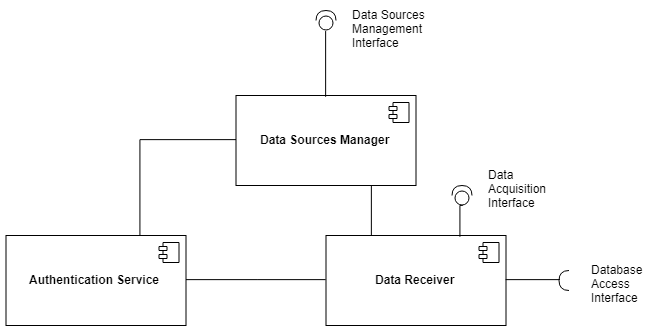
\includegraphics[width=0.8\columnwidth]{rcv1.png}
		\caption{Basic data acquisition functions}
	\end{subfigure}%
	~ 
	\begin{subfigure}[t]{0.5\textwidth}
		\centering
		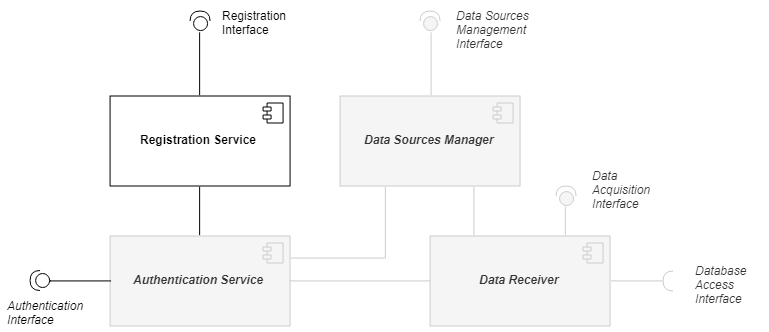
\includegraphics[width=\columnwidth]{rcv2.png}
		\caption{Authentication and registration}
	\end{subfigure}
	
	\caption{Data Acquisition Module development}
\end{figure*}
\FloatBarrier

\FloatBarrier
\begin{figure*}[ht!]
	\centering
	\begin{subfigure}[t]{0.5\textwidth}
		\centering
		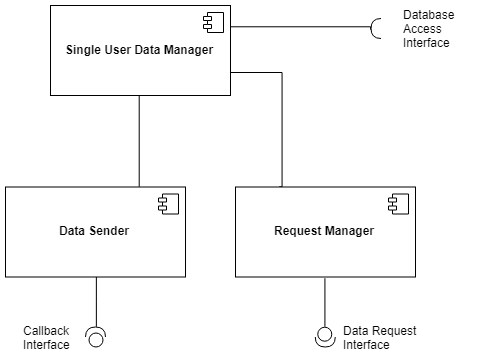
\includegraphics[width=0.8\columnwidth]{snd1.png}
		\caption{Single Data requests}
	\end{subfigure}%
	~ \vspace{20px}
	\begin{subfigure}[t]{0.5\textwidth}
		\centering
		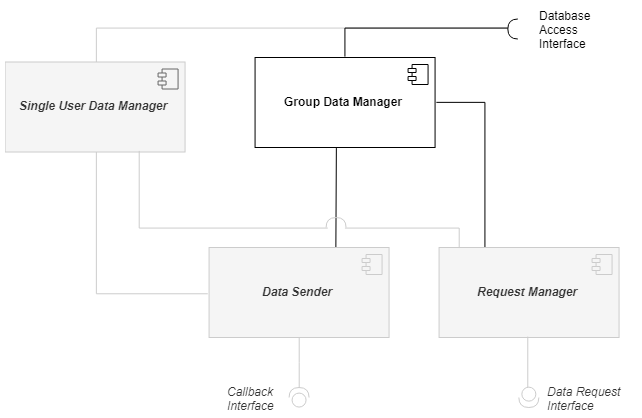
\includegraphics[width=\columnwidth]{snd2.png}
		\caption{Group Data requests}
	\end{subfigure}

	\begin{subfigure}[t]{0.8\textwidth}
		\centering
		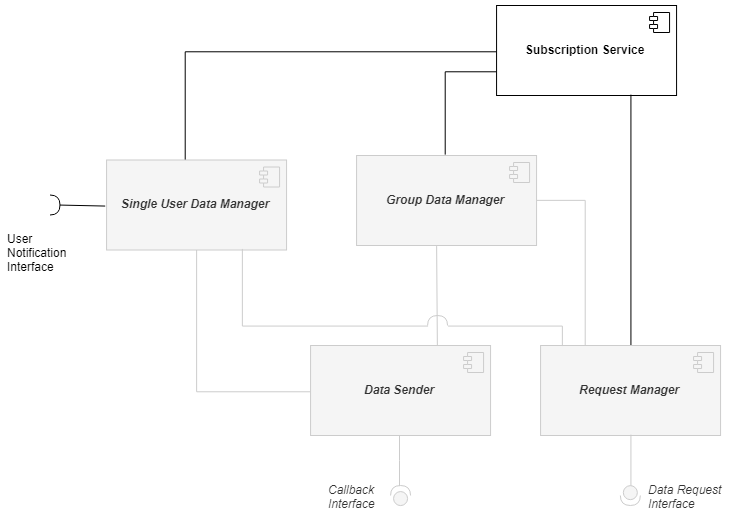
\includegraphics[width=\columnwidth]{snd3.png}
		\caption{Subscription functionalities}
	\end{subfigure}
	
	\caption{Data Request Module development}
\end{figure*}
\FloatBarrier

\subsubsection{AutomatedSOS}
Prima BE, poi external Interfaces, poi FE

\subsubsection{Track4Run}
Prima BE, poi external Interfaces, poi FE

\subsection{Integration and Testing}
\subsubsection{Entry Criteria}
Percentuali (?)
Di base, quando i back end sono completati a meno di autenticazione

\subsubsection{Elements to be Integrated}

\FloatBarrier
\begin{figure*}[ht!]
	\centering
	\begin{subfigure}[t]{0.5\textwidth}
		\centering
		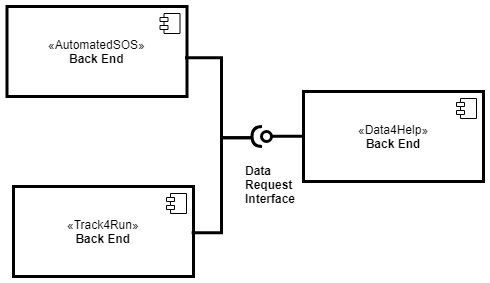
\includegraphics[width=0.7\columnwidth]{sysInt1.png}
		\caption{Back-ends integration}
	\end{subfigure}%
	~ 
	\begin{subfigure}[t]{0.5\textwidth}
		\centering
		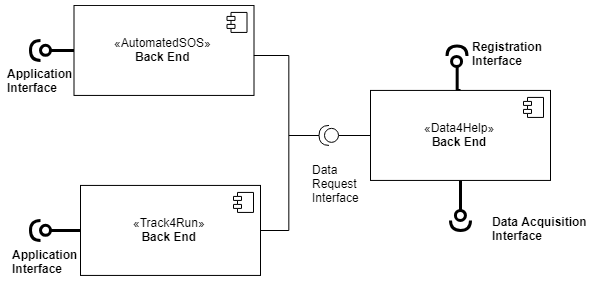
\includegraphics[width=\columnwidth]{sysInt2.png}
		\caption{External Interfaces integration}
	\end{subfigure}

	\caption{Subsystem Integration}
\end{figure*}
\FloatBarrier

\FloatBarrier
\begin{figure}[!h]
	\centering
	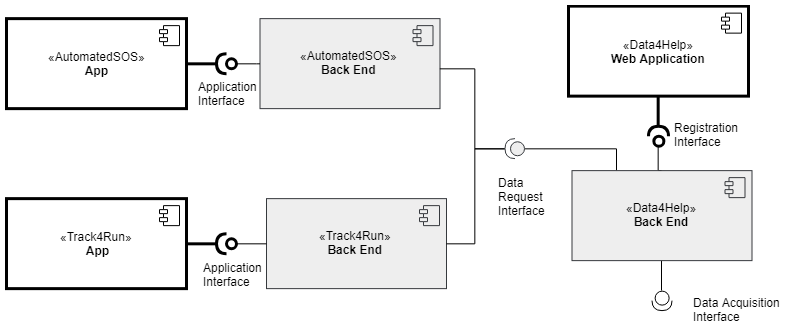
\includegraphics[width=0.8\columnwidth]{sysInt3.png}
	\caption{Front-ends integration}
\end{figure}

\FloatBarrier

\FloatBarrier
\begin{figure}[!h]
	\centering
	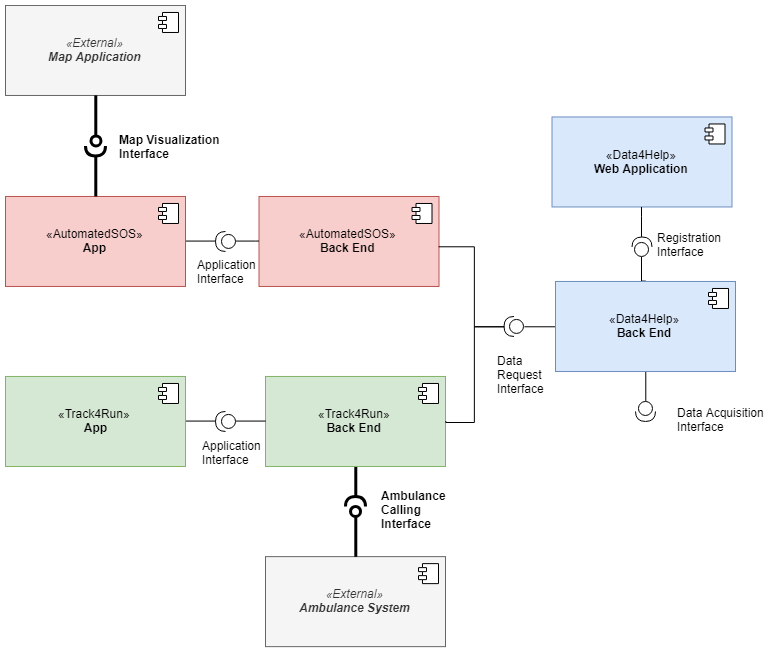
\includegraphics[width=\columnwidth]{sysInt4.png}
	\caption{External Services integration}
\end{figure}

\FloatBarrier


\subsubsection{Integration Testing Strategy}
bottom up o continuous integration?

\subsubsection{Sequence of Component/Function Integration}

componente per componente?
